\section{Introduction}
\stepcounter{subsection} %We don't use subsection titles, only frametitles
\label{sec:introduction}

%---------------------------------------------------------------
% 1. Seminar outline
%---------------------------------------------------------------
\begin{frame}{Our goals for today}
    
    \begin{columns}[t]
    \column{.45\textwidth}
        \begin{enumerate}
            \item Tell you about the course
            \item Introduce `open science'
            \item Share experiences of COVID-19
        \end{enumerate}

    \column{.45\textwidth}
        \begin{figure}
            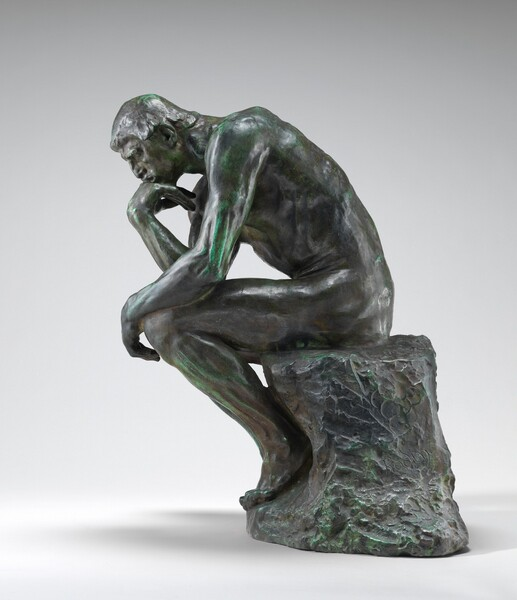
\includegraphics[width=0.8\textwidth]{images/the_thinker_NPA_1942_5_12.jpg}
            \givecredit{\centering Image courtesy \textlink{https://www.nga.gov/collection/art-object-page.1005.html}{National Gallery of Art, Washington}.}
        \end{figure}
    \end{columns}
\end{frame}

%---------------------------------------------------------------
% 2. People
%---------------------------------------------------------------

\begin{frame}{Who's here?}
    
    \begin{columns}[t]
    \column{.3\textwidth}
    
    \begin{block}{Andy Clifton}
    \centering
    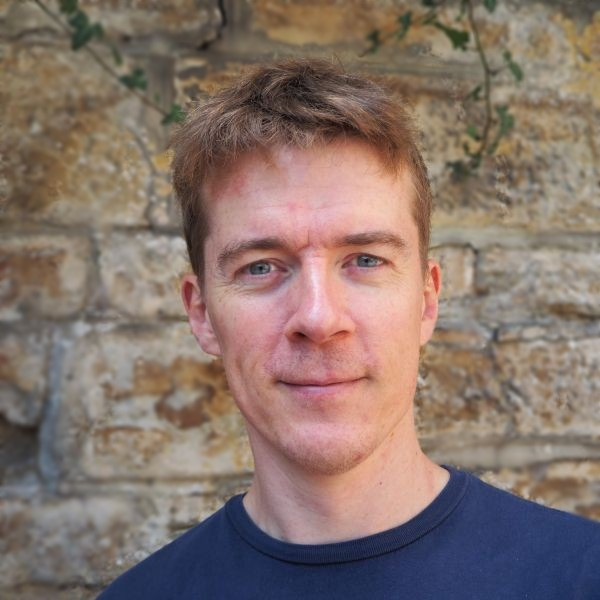
\includegraphics[width=0.8\textwidth]{images/Clifton_Headshot_2019_600W_600H_blur.jpg}\\
    IEA Wind Task 32 Operating Agent \\
    \orcid{0000-0001-9698-5083}
    \linkedin{http://www.linkedin.com/in/andyclifton}
    \end{block}
   
    \column{.3\textwidth}
    \begin{block}{Nikola Vasiljevic}
    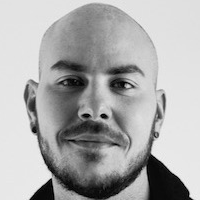
\includegraphics[width=0.8\textwidth]{images/Vasiljevic_Headshot.png}\\
    Special Consultant for Digitalization \\
    \orcid{0000-0002-9381-9693}
    \linkedin{https://dk.linkedin.com/in/niva83}
    \end{block}
    
    \column{.3\textwidth}
    
    \begin{block}{And you}
    
    \centering
    {\fontsize{100}{120}\selectfont\faUsers}\\
    Please introduce yourselves!
    
    \end{block}
    
    \end{columns}


\end{frame}


